\begin{frame}
\frametitle{P2P Networks}
\framesubtitle{Characteristics}
\begin{table}
\begin{tabular}{p{7cm}p{3cm}}
\begin{itemize}
  \item Scalable
  \item Decentralized
  \item Self-maintained
  \item Robust
\end{itemize}
&
\vspace{1.5cm}
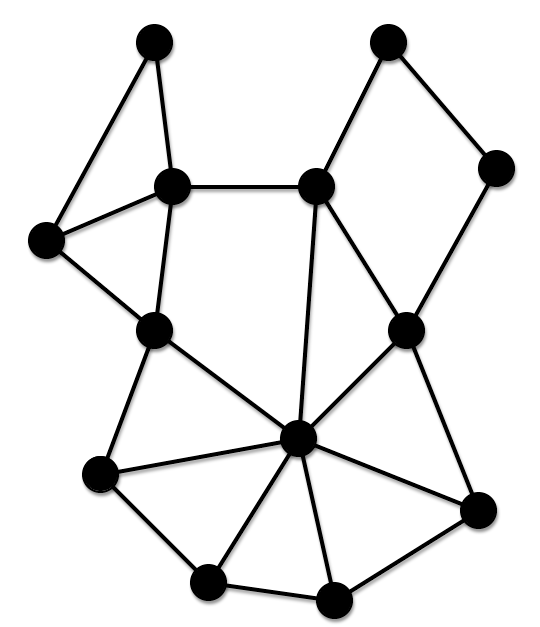
\includegraphics[width=4cm]{img/p2p-unstructured}\\
\end{tabular}
\end{table}
\end{frame}

\begin{frame}
\frametitle{P2P Networks}
\framesubtitle{Overlay structure}
\begin{table}
\begin{tabular}{p{7cm}p{3cm}}
\begin{itemize}
    \item Structured networks (CAN, CHORD)
    \item Unstructured networks (Gnutella, Bittorrent)

\end{itemize}
&
\vspace{1.5cm}
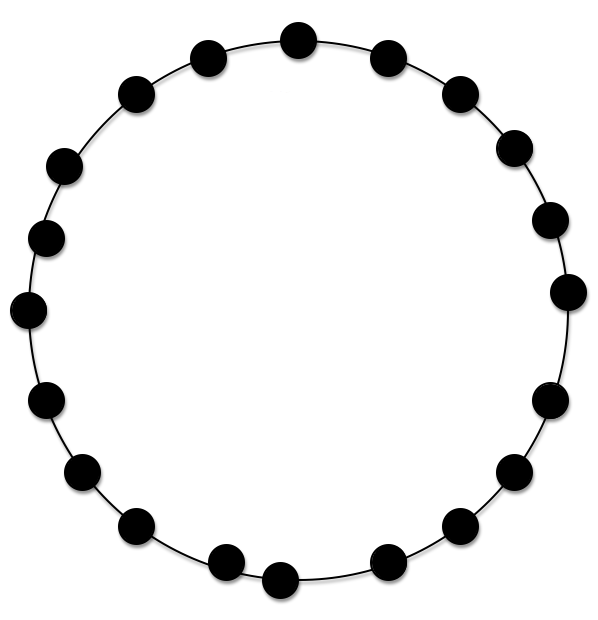
\includegraphics[width=4cm]{img/p2p-structured}\\
\end{tabular}
\end{table}
\end{frame}

\begin{frame}
\frametitle{P2P Networks}
\framesubtitle{The problem}
\begin{table}
\begin{tabular}{p{7cm}p{3cm}}
\begin{itemize}
  \item P2P Networks only identify the nodes by their IP address 
\end{itemize}
&
\vspace{1.5cm}
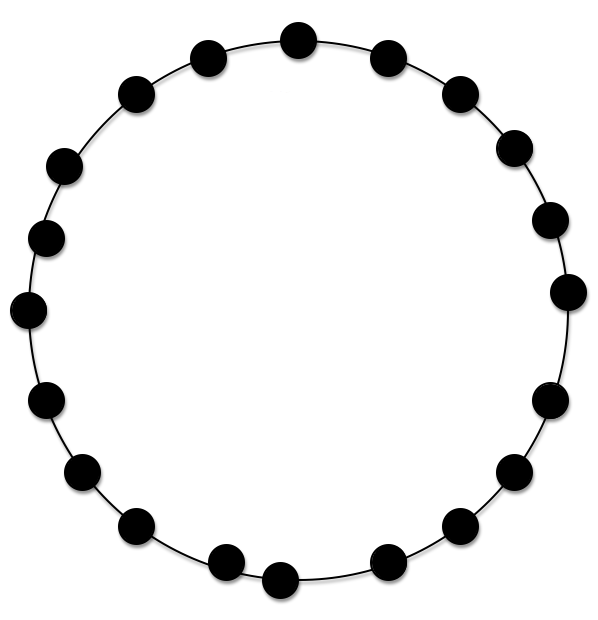
\includegraphics[width=4cm]{img/p2p-structured}\\
\end{tabular}
\end{table}
\end{frame}

%- Problema
\begin{frame}
\frametitle{The problem (2)}
%\framesubtitle{Characteristics}
\begin{table}
\begin{tabular}{p{7cm}p{3cm}}
\begin{itemize}
  \item Existing systems manage \textbf{user-level permission} by issuing \textbf{pre-shared keys}.
  \item This does \textbf{not provide the flexibility} that a username-password based identification provides.
\end{itemize}
&
\vspace{1.5cm}
%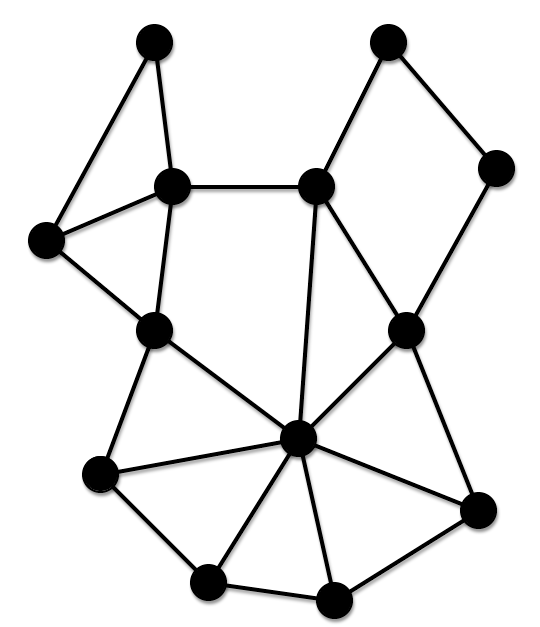
\includegraphics[width=4cm]{img/p2p-unstructured}\\
\begin{itemize}
  \item Access from \textbf{Multiple devices}?
  \item \textbf{Key handling}
\end{itemize}
\end{tabular}
\end{table}
\end{frame}


\begin{frame}
\frametitle{The problem (3)}
%\framesubtitle{Characteristics}
\begin{table}
\begin{tabular}{p{7cm}p{3cm}}
\begin{itemize}
  \item The use of a \textbf{username and a password} means that the \textbf{user keys} needs to be \textbf{secured inside} the identification system
  \item While a \textbf{solution} has been proposed before, it does \textbf{not} take in
consideration the presence of \textbf{malicious nodes}
\end{itemize}
&
\vspace{1.5cm}
%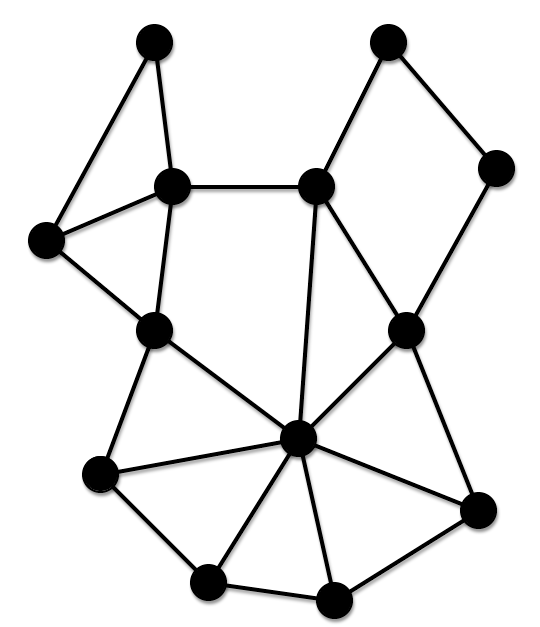
\includegraphics[width=4cm]{img/p2p-unstructured}\\
\end{tabular}
\end{table}
\end{frame}

\begin{frame}
%- Porque el problema es importante
\frametitle{Why this is important?}
%  - Redes p2p solo identifican nodos-ip
%  - Explicar redes estructuradas para ello
%  - Necesario si es que uno quiere construir aplicaciones que requieran
%    permisos a nivel de usuario
%\framesubtitle{Characteristics}
\begin{table}
\begin{tabular}{p{7cm}p{3cm}}
\begin{itemize}
  \item \textbf{Applications that need user-level permissions need a way to identify users}
\end{itemize}
&
\vspace{1.5cm}
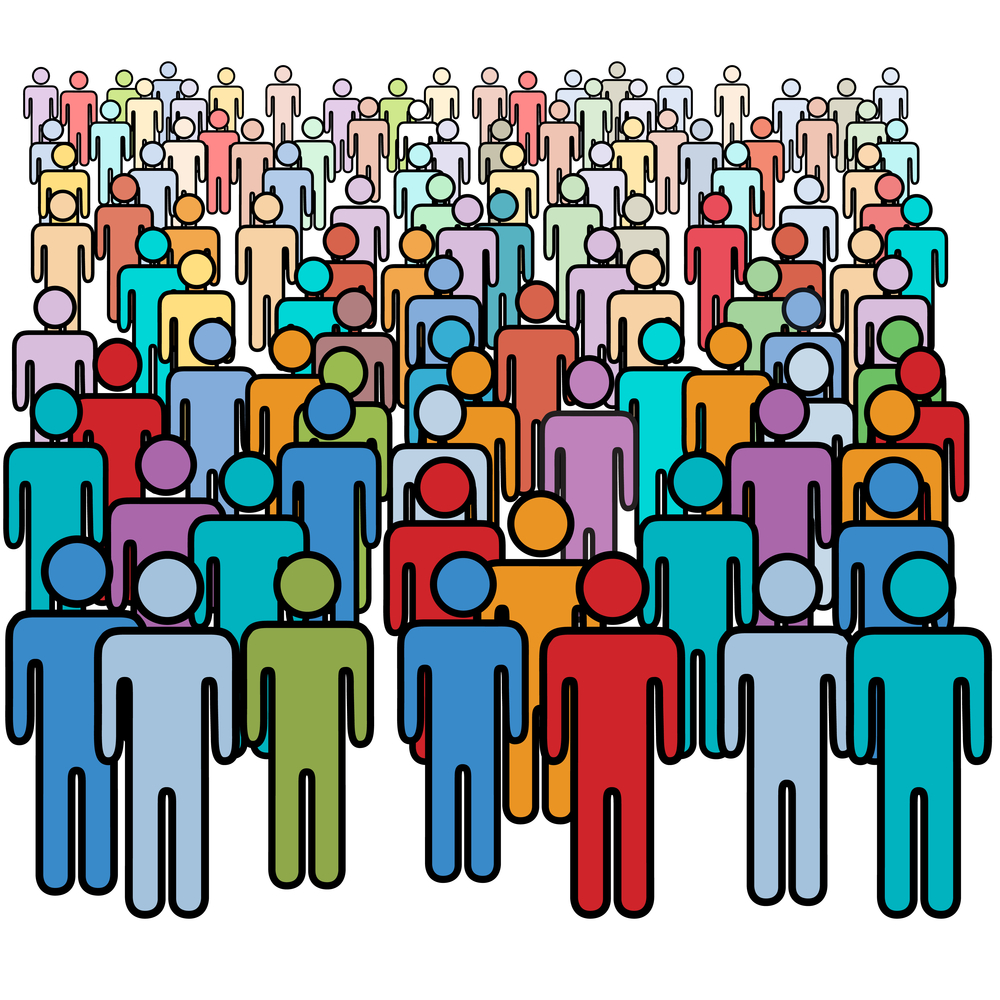
\includegraphics[width=4cm]{img/users}\\
\end{tabular}
\end{table}
\end{frame}



\begin{frame}
\frametitle{Goals}
%\framesubtitle{Characteristics}
\begin{table}
\begin{tabular}{p{7cm}p{3cm}}
\begin{itemize}
  \item Analize the security risks in using username/password identification in P2P networks. 
  \item Check the different security schemes that can be used in a P2P network with malicious nodes.
  \item Propose a P2P username/password identification system.
\end{itemize}
&
\vspace{1.5cm}
%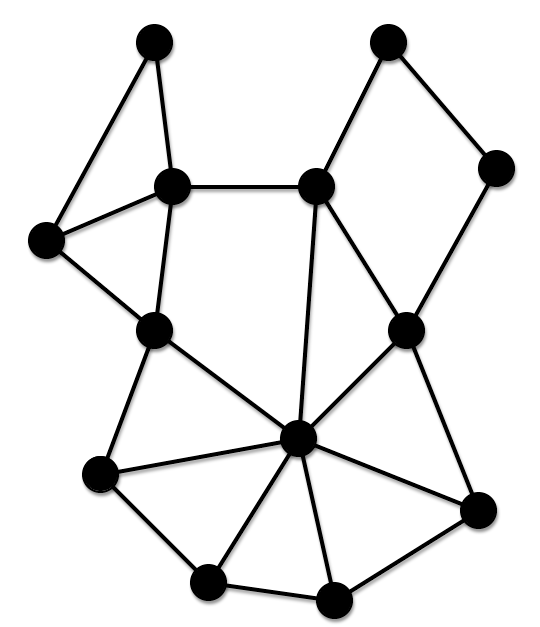
\includegraphics[width=4cm]{img/p2p-unstructured}\\
\end{tabular}
\end{table}
\end{frame}
